\scanpage{124}
le foncteur compatible aux $\otimes$ associatifs unitaires qu'on obtient de $C$ dans $\mathrm{Rep}_k(G)$, et voir en particulier sous quelles conditions il est une équivalence de catégories: \deleted{Alors}\inserted{\handwritten{il f. et \unsure{p.|s.} que $A$ soit commutatif! ``Géométriquement''}\handwritten{\begin{tikzpicture}[x=.4cm,y=.4cm,baseline=-.2ex]\draw (0,-.55) .. controls (-.12,.02) and (.12,.28) .. (.42,.30)--(6.8,.30) .. controls (7.04,.30) and (7.18,.36) .. (7.18,.54);\end{tikzpicture}}} Lorsqu'il en est ainsi,\inserted{\handwritten{\uuline{dans le cas gradué anticomm.}}\handwritten{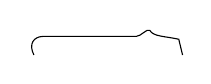
\begin{tikzpicture}[x=.4cm,y=.4cm,baseline=-.2ex]\draw (0,-.30) .. controls (-.18,.06) and (0,.28) .. (.28,.29)--(3.25,.29) .. controls (3.40,.29) and (3.58,.55) .. (3.68,.48) .. controls (3.80,.28) and (4.15,.30) .. (4.60,.20)--(4.72,-.30);\end{tikzpicture}}} \deleted{k}la situation est décrite entièrement par la donnée de $G$, de la graduation sur \deleted{son} le foncteur oubli sur \deleted{$C$}\inserted{$R_k(G)$\handwritten{\begin{tikzpicture}[x=.4cm,y=.4cm,baseline=-.2ex]\draw (0,-.48) .. controls (-.12,.0) and (.15,.12) .. (.42,.14)--(1.38,.14) .. controls (1.56,.16) and (1.64,.24) .. (1.65,.43);\end{tikzpicture}}}, décrite par un homomorphisme de monoïdes $\underline{G}_m\handwritten{\to}G$, et enfin la condition que pour deux représentation $M,N$ de $G$, l'isomorphisme de Koszul $M\otimes N\handwritten{\xrightarrow{\sim}}N\otimes M$ sur les vectoriels sous-jacents est compatible avec l'action de $G$. Bien sûr, si $k$ est de car 2, ce n'est pas une restriction, et dans ce cas d'ailleurs Koko ne change rien i.e. tous nos ennuis et distinguos disparaissent. \deleted{Si} Il suffit en tous cas que l'homomorphisme induit $\handwritten{\mu}_2\handwritten{\longrightarrow}G$ soit central;\inserted{\handwritten{et on voit que \unsure{cela est forcé|cel. est forcé|cela \deleted{est}vérifié|\deleted{cela est} vérifié} \unsure{si|et} (car $k\ne2$, \unsure{c.c.|c.q.|c.f.}) que cela implique $A^{\unsure{*|\#}}=A^{\unsure{\oplus|0|\overline{0}}}$ donc $A^*$ commutatif !}\handwritten{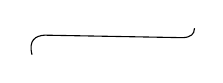
\begin{tikzpicture}[x=.4cm,y=.4cm,baseline=-.2ex]\draw (0,-.42) .. controls (-.12,.05) and (.12,.18) .. (.40,.20)--(4.80,.12) .. controls (5.04,.14) and (5.15,.22) .. (5.16,.42);\end{tikzpicture}}} à fortiori\inserted{\handwritten{il suffit}\handwritten{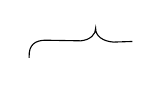
\begin{tikzpicture}[x=.4cm,y=.4cm,baseline=-.2ex]\draw (0,-.34) .. controls (-.03,.10) and (.22,.21) .. (.50,.22)--(1.64,.20) .. controls (1.94,.23) and (2.12,.41) .. (2.11,.60) .. controls (2.10,.35) and (2.35,.18) .. (2.68,.16)--(3.28,.18);\end{tikzpicture}}} que $\underline{G}_m\handwritten{\to}G$ soit central\handwritten{,}\unsure{.|\deleted{,}}\deleted{i.e.}\margin{\deleted{\handwritten{et on \unsure{voit}}}}\inserted{Cela signifie\handwritten{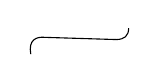
\begin{tikzpicture}[x=.4cm,y=.4cm,baseline=-.2ex]\draw (0,-.40) .. controls (-.08,.05) and (.17,.16) .. (.46,.13)--(2.72,.06) .. controls (2.98,.07) and (3.10,.17) .. (3.11,.42);\end{tikzpicture}}} que la décomp\deleted{\unsure{e|s}}o\deleted{\unsure{o|e}}s\deleted{t}ition d'un $M$ en composants \deleted{homogènes}\inserted{pairs et impair\handwritten{s}\handwritten{
\begin{tikzpicture}[x=.4cm,y=.4cm,baseline=-.2ex]\draw (0,-.20)--(2.20,-.26) .. controls (2.42,-.26) and (2.58,-.12) .. (2.57,.04);\end{tikzpicture}}} soit invariante sous $G$ i.e. se fasse dans $C$,\deleted{e}resp. qu'il en soit de même pour la décomposition en degrés\inserted{\handwritten{entiers}\handwritten{\begin{tikzpicture}[x=.4cm,y=.4cm,baseline=-.2ex]\draw (0,-.30) .. controls (.15,.08) and (.35,.14) .. (.53,.14)--(1.92,.12) .. controls (2.12,.13) and (2.23,.25) .. (2.20,.42);\end{tikzpicture}}}. Noter que cette dernière condition s'exprime directement en termes de $C$ (muni de sa structure $\otimes$ et du foncteur \deleted{oubli} gradué\deleted{\unsure{f|i|)|s|x}} $C\handwritten{\to}\mathrm{Grdf}(k)$), \deleted{et \deleted{i}on \deleted{espère}\inserted{\handwritten{voit}} que cette condition est suffisante (peut-être nécessaire et suffisante)\inserted{\handwritten{si car. $k\ne2$}\handwritten{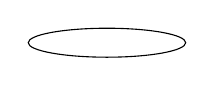
\begin{tikzpicture}[x=.4cm,y=.4cm,baseline=-.2ex]\draw (0,0) ellipse (2.5 and .46);\end{tikzpicture}}} pour qu'on soit dans le cas favorable\inserted{\handwritten{\unsure{où|si}}\handwritten{\begin{tikzpicture}[x=.4cm,y=.4cm,baseline=-.2ex]\draw (0,.15) .. controls (.35,.21) and (.56,.13) .. (.64,-.18) .. controls (.70,-.36) and (.91,-.40) .. (1.14,-.40);\end{tikzpicture}}} $C\handwritten{\to}\mathrm{Rep}_k(G)$ \unsure{\deleted{soit}\inserted{\handwritten{est}}|\deleted{soi}\handwritten{es}t|soit} une équivalence.}
\margin{\handwritten{\begin{tikzpicture}[x=.4cm,y=.4cm,baseline=-.2ex]\draw (.18,.42) .. controls (-.05,.46) and (-.08,.25) .. (.01,.02) .. controls (.13,-.30) and (.44,-.34) .. (.68,-.27);\end{tikzpicture}}}


\handwritten{1\unsure{\deleted{-}0|0})} Ce résultat s'appliquera alors, en particulier, à la catégorie des motifs\inserted{s\deleted{m}emi-simples\handwritten{\begin{tikzpicture}[x=.4cm,y=.4cm,baseline=-.2ex]\draw (0,-.40) .. controls (-.05,.06) and (.16,.17) .. (.45,.18)--(2.63,.15) .. controls (2.88,.16) and (3.03,.29) .. (3.02,.49);\end{tikzpicture}}} (car les \deleted{foncteurs} graduations naturelles sur les foncteurs $H^\bullet$ qu'on arrive à y définir \deleted{sont} proviennent d'une graduation de la catégorie des motifs, - ce qui n'est qu'une traduction du fait que les correspondances\inserted{cohomologiques\handwritten{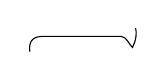
\begin{tikzpicture}[x=.4cm,y=.4cm,baseline=-.2ex]\draw (0,-.34) .. controls (-.05,.05) and (.16,.14) .. (.42,.14)--(2.90,.14) .. controls (3.08,.13) and (3.15,-.12) .. (3.26,-.21) .. controls (3.38,.03) and (3.40,.25) .. (3.36,.40);\end{tikzpicture}}} de Kunneth sur une variété algébrique projective lisse sont algébriques). On \deleted{e}respire ! Mais on fera attention que les foncteurs $H^\bullet$ en question ne sont pas des foncteurs fibres proprement, mais des foncteurs fibres tordus.(On ne pourra s'empêcher de les appeler quand-même foncteurs fibres!) Quand on travaille avec des motifs pas nécess\deleted{i}airement
